\section{Applications}

 \frame{\sectionpage}

\begin{frame}{Design Estimators}
    The goal: Make the confidence intervals \textcolor{mygreen}{\textbf{shorter}}
    \begin{align*}
        \hat{\tau}_{\gamma}&\pm l_{\alpha}, &l_{\alpha}&=\min\left\{ l:\mathbf{P}\left[\left|b+n^{-\frac{1}{2}}\hat{V}_{\gamma}^{\frac{1}{2}}\tilde{Z}\right|\leq l\right]\geq1-\alpha,\forall\left|b\right|\leq\hat{B}_{\gamma,M}\right\} 
    \end{align*}

    by minimizing the worst-case MSE of
    $$
    \hat{\tau}= \hat{\mu}_{\gamma,+}- \hat{\mu}_{\gamma,-}=\frac{\sum_{i}\gamma_{+}\left(Z_{i}\right)Y_{i}}{\sum_{i}\gamma_{+}\left(Z_{i}\right)} - \frac{\sum_{i}\gamma_{-}\left(Z_{i}\right)Y_{i}}{\sum_{i}\gamma_{-}\left(Z_{i}\right)}
    $$
\end{frame}

\begin{frame}{Design Estimators: Quadratic Programming}
    Solve
    $$
    \min_{\gamma_{\pm}\left(\cdot\right)}\frac{1}{n}\left( \textcolor<2>{mygreen}{\int\gamma_{-}^{2}\left(z\right)\mathrm{d}\bar{F}\left(z\right)+\int\gamma_{+}^{2}\left(z\right)\mathrm{d}\bar{F}\left(z\right)} \right)+\left(t_{1}+t_{2}\right)^{2}
    $$
    \only<2>{
        Using the fact
        $$
        \mathrm{Var}\left[\gamma_{\diamond}(Z_i)Y_i\right] \leq \int \gamma_{\diamond}^2(z)\mathrm{d}F(z),\ \diamond\in\{+,-\}
        $$
    }
    \only<3->{s.t.
    {\small
        \begin{align*}
        \left|h\left(u,\gamma_{+}\right)-h\left(u,\gamma_{-}\right)\right| & \leq t_{1}, & \forall u &  & \uncover<4->{\text{confounding bias}}\\
        M\left|h\left(u,\gamma_{\diamond}\right)-\bar{w}\left(u\right)\right| & \leq t_{2}, & \forall u,\diamond\in\left\{ \pm\right\}  &  & \uncover<4->{\text{CATE-hetrogeneity bias}}\\
        \int\gamma_{+}\left(z\right)\mathrm{d}\bar{F}\left(z\right)=\int\gamma_{-}\left(z\right)\mathrm{d}\bar{F}\left(z\right) & =1 &  &  & \uncover<5->{\text{normalization constraint}} \\
        \gamma_{-}\left(z\right) & =0, & z\geq c &  & \uncover<5->{\text{Sharp RD}} \\
        \gamma_{+}\left(z\right) & =0, & z<c\\
        \left|\gamma_{\diamond}\left(z\right)\right| & \leq Cn^{\beta}, & \forall z,\diamond\in\left\{ \pm\right\}  &  & \uncover<6->{\text{no observation is given excessive influence}}
    \end{align*}}}
        
\end{frame}

\begin{frame}{Design Estimators: Quadratic Programming}
    Solve
    $$
    \min_{\gamma_{\pm}\left(\cdot\right)}\frac{1}{n}\left( {\int\gamma_{-}^{2}\left(z\right)\mathrm{d}\textcolor<2>{mygreen}{\bar{F}}\left(z\right)+\int\gamma_{+}^{2}\left(z\right)\mathrm{d}\textcolor<2>{mygreen}{\bar{F}}\left(z\right)} \right)+\left(t_{1}+t_{2}\right)^{2}
    $$
    s.t.
    {\small
        \begin{align*}
        M\left|h\left(u,\gamma_{\diamond}\right)-\textcolor<2>{mygreen}{\bar{w}}\left(u\right)\right| & \leq t_{2}, & \forall u,\diamond\in\left\{ \pm\right\}  &  & {\text{CATE-hetrogeneity bias}}\\
        \int\gamma_{+}\left(z\right)\mathrm{d}\textcolor<2>{mygreen}{\bar{F}}\left(z\right)=\int\gamma_{-}\left(z\right)\mathrm{d}\textcolor<2>{mygreen}{\bar{F}}\left(z\right) & =1 &  &  & {\text{normalization constraint}}
    \end{align*}}

    \uncover<2->{
        \small
        \begin{align*}
            &\bar{F}(\cdot): &F_{G}\left(t\right) &= \int\mathbf{1}\left(\left\{ z\leq t\right\} \right)\int p\left(z\mid u\right)\mathrm{d}G\left(u\right)\mathrm{d}\lambda\left(z\right) \\
            &\bar{w}(\cdot): &\tau_{w}&= \int\frac{w\left(u\right)}{\mathbb{E}_{G}\left[w\left(U\right)\right]}\tau\left(u\right)\mathrm{d}G\left(u\right)
        \end{align*}
    }
\end{frame}

\begin{frame}{Design Estimators: Quadratic Programming}

    {
        \small
        \begin{align*}
            &\bar{F}(\cdot): &F_{G}\left(t\right) &= \int\mathbf{1}\left(\left\{ z\leq t\right\} \right)\int p\left(z\mid u\right)\mathrm{d}G\left(u\right)\mathrm{d}\lambda\left(z\right) \\
            &\bar{w}(\cdot): &\tau_{w}&= \int\frac{w\left(u\right)}{\mathbb{E}_{G}\left[w\left(U\right)\right]}\tau\left(u\right)\mathrm{d}G\left(u\right)
        \end{align*}
    }

    \begin{itemize}
        \item $\bar{F}\left(\cdot\right)$ assigns non-trivial mass to $\left[c,\infty\right)$ and $\bar{w}(\cdot)$ is bounded: $\exists k>1$ s.t.
        $$\mathbb{P}\left[\frac{1}{k}<\bar{F}\left(\left[c,\infty\right)\right)<1-\frac{1}{k},\sup_{u}\left|\bar{w}\left(u\right)\right|<k\right]\xrightarrow{n\rightarrow\infty}1$$
        \item $\int\gamma_{\diamond}^{\left(n\right)}\left(z\right)\mathrm{d}F\left(z\right)$ is asymptotically lower bounded by a strictly positive number: $$\exists\delta>0\text{ s.t. } \mathbb{P}\left[\int\gamma_{\diamond}^{\left(n\right)}\left(z\right)\mathrm{d}F\left(z\right)>\delta\right]\xrightarrow{n\rightarrow\infty}1$$
    \end{itemize}
    
\end{frame}

\begin{frame}{Design Estimators: Quadratic Programming}
    $$
    \begin{aligned}
        \frac{1}{k}<\bar{F}\left(\left[c,\infty\right)\right)<1-\frac{1}{k},\sup_{u}\left|\bar{w}\left(u\right)\right| &<k\\
        \int\gamma_{\diamond}^{\left(n\right)}\left(z\right)\mathrm{d}F\left(z\right) &>\delta
    \end{aligned}\Rightarrow 
    \begin{aligned}
        &\sup_{z}\left|\gamma_{\diamond}^{\left(n\right)}\left(z\right)\right| <Cn^{\beta}  \mathbb{E} \left[\gamma_{\diamond}^{\left(n\right)}\left(Z_{i}\right)\right]\\
        &\sup_{u}\left|h\left(u,\gamma_{\diamond}^{\left(n\right)}\right)\right| <C'\mathbb{E}\left[\gamma_{\diamond}^{\left(n\right)}\left(Z_{i}\right)\right]
    \end{aligned}\uncover<2>{\Rightarrow}
    $$

    \only<2>{\begin{block}{\textbf{Theorem: Asymptotic Normality of $\hat{\tau}$}}
        \small
        Suppose the sequence of weighting kernels $\gamma_{+}^{\left(n\right)}$ and $\gamma_{-}^{\left(n\right)}$ is deterministic, and  $\exists\beta\in\left(0,\frac{1}{2}\right), C,C'>0$ s.t. $\forall n$ large enough: $\sup_{z}\left|\gamma_{\diamond}^{\left(n\right)}\left(z\right)\right| <Cn^{\beta}  \mathbb{E} \left[\gamma_{\diamond}^{\left(n\right)}\left(Z_{i}\right)\right]$, $\sup_{u}\left|h\left(u,\gamma_{\diamond}^{\left(n\right)}\right)\right| <C'\mathbb{E}\left[\gamma_{\diamond}^{\left(n\right)}\left(Z_{i}\right)\right]$ where $\diamond=\left\{ +,-\right\}$
        Then 
        $$
        \frac{\sqrt{n}\left(\hat{\tau}_{\gamma}-\theta_{\gamma}\right)}{\sqrt{V_{\gamma}}}\xrightarrow{d}\mathcal{N}\left(0,1\right)
        $$
    \end{block}}
\end{frame}

\begin{frame}{Design Estimators: Procedure}

    \begin{itemize}
        \item<1-> \textcolor{mygreen}{\textbf{Input:}}
        \begin{itemize}
            \item[-] samples $ \left\{ Z_{i},Y_{i},W_{i}\right\} $ and cutoff $c$
            \item[-] sensitivity model $\mathcal{T}_{M}$, estimand of interest $\tau_{w}$
            \item[-] nominal significance level $\alpha$ 
        \end{itemize}

        \item<2-> \textcolor{mygreen}{\textbf{Procedure:}}
        \begin{itemize}
            \item[S1] guess/estimate $\bar{F}\left(\cdot\right)$ and $\bar{w}\left(\cdot\right)$ via nonparametric maximum likelihood
            \item[S2] solve the minimax program, get $\gamma_{+},\gamma_{-}$ 
            \item[S3] form the point estimate $\hat{\tau}_{\gamma}$ and its variance $\hat{V}_{\gamma}$
            \item[S4] estimate the worst-case bias $\hat{B}_{\gamma}=\sup\left\{ \left|\mathrm{Bias}\left[\gamma_{\pm},\tau_{w};\alpha_{0}\left(\cdot\right),\tau\left(\cdot\right),G\right]\right|:G\in\mathcal{G}_{n},\alpha_{\left(0\right)}\left(\cdot\right)\in\left[0,1\right],\tau\left(\cdot\right)\in\mathcal{T}_{M}\right\} $
            \item[S5] form the bias-aware CIs at level $\alpha$ as $\hat{\tau}_{\gamma}\pm l_{\alpha},l_{\alpha}=\min\left\{ l:\mathbf{P}\left[\left|b+n^{-\frac{1}{2}}\hat{V}_{\gamma}^{\frac{1}{2}}\tilde{Z}\right|\leq l\right]\geq1-\alpha,\forall\left|b\right|\leq\hat{B}_{\gamma,M}\right\} $
        \end{itemize}
    \end{itemize}
    
\end{frame}

\begin{frame}{Design Estimators: Example}
    \begin{figure}\label{fig:example}
        \centering
        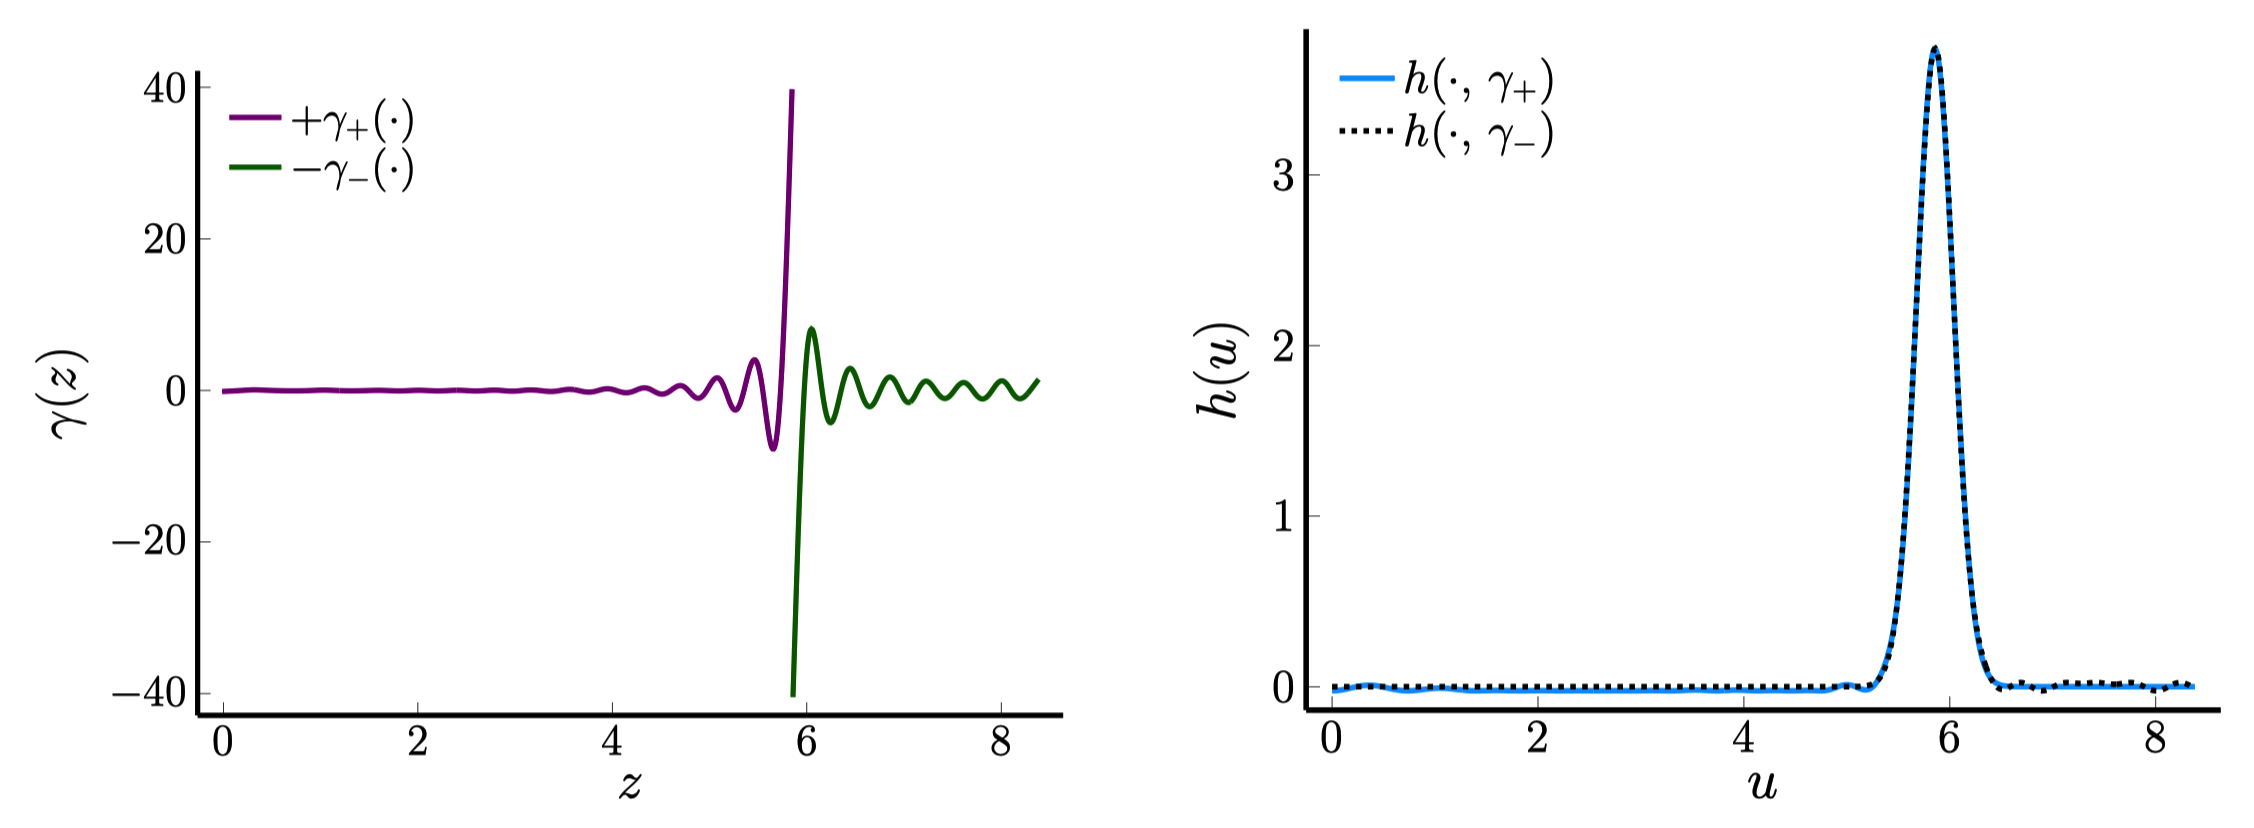
\includegraphics[height = 0.65 \textheight]{images/fig1.png}
        \end{figure}
\end{frame}